\documentclass[a4paper,12pt]{article}
\usepackage[utf8]{inputenc}
\usepackage{hyperref}
\usepackage{graphicx}
\usepackage{float}
\graphicspath{ {images/} }

\begin{document}

\begin{titlepage}

\newcommand{\HRule}{\rule{\linewidth}{0.5mm}} % Defines a new command for the horizontal lines, change thickness here

\center % Center everything on the page
 
%----------------------------------------------------------------------------------------
%-	HEADING SECTIONS
%----------------------------------------------------------------------------------------
\begin{center}
	
\includegraphics[width=7cm]{../Images/SavageRus.png}
\end{center}	
\vfill
\textsc{\LARGE University of Pretoria}\\[1.5cm]
\textsc{\Large COS 301 - Software Engineering}\\[0.5cm]
\textsc{\large The Savage Ru's}\\[0.5cm]

%----------------------------------------------------------------------------------------
%-	TITLE SECTION
%----------------------------------------------------------------------------------------

\HRule \\[0.4cm]
{ \huge \bfseries VizARD Architectural and Functional Specification - Version 0.3}\\[0.4cm] % Title of your document
{\large \today}
\HRule \\[1.5cm]
 
%----------------------------------------------------------------------------------------
%-	AUTHOR SECTION
%----------------------------------------------------------------------------------------

\begin{minipage}{0.4\textwidth}
\begin{flushleft} \large
\emph{Author(s):}\\
Jodan \textsc{Alberts}\\ % Your name
Mark \textsc{Klingenberg}\\
Una \textsc{Rambani}\\
Ruan \textsc{Klinkert}\\
\end{flushleft}
\end{minipage}
~
\begin{minipage}{0.4\textwidth}
\begin{flushright} \large
\emph{Student number(s):} \\
14395283\\ % Student number
14020272\\
14004489\\
14022282\\

\end{flushright}
\end{minipage}\\[4cm]

 % Date, change the \today to a set date if you want to be precise

 
%----------------------------------------------------------------------------------------

\vfill % Fill the rest of the page with whitespace

\end{titlepage}

\newpage

\tableofcontents

\newpage

\section{Introduction}

This is the software requirements specification for the vizARD Augmented Reality application that is being developed for EPI-USE Labs.
\newline
VizARD is a mobile application that allows for quick and easy visualization of tabular data.

\section{Vision and Background}
The system will allow a user to:
\begin{itemize}
\item Take a picture of a table of numerical data
\item Use OCR (Optical Character Recognition) to read the data from the picture
\item Generate an appropriate graph for the data
\item View a 3D model of this graph through Augmented Reality
\end{itemize}   . 
\newline
Additionally, the system will allow users to send images (or screen captures) of generated graphs to other devices via popular social media channels.

\newpage
\section{Software Architecture}
\subsection{Architectural Scope}
ViZARD is a partially online application, because a small amount of processing happens remotely. The local application will run entirely as a Unity3D application. After an image has been taken by the user, it is sent in a POST request to the OpenOCR API server for Tesseract to process. The results are returned and parsed into a C\# object where our beautifully engineered scripts handle the graph generation.

\subsection{Integration and Access Channel Requirements}
\begin{itemize}
\item The system accesses the OpenOCR server by each local deployment through a RESTful API which will require internet access.
\item  Since the application is being developed entirely in Unity3D (save for the OCR), Unity selects the APIs to complete tasks such as file system access, camera access and network access.
\item End users will be able to access the system through mobile applications made available for Android and iOS operating systems.
\end{itemize}

\subsection{Quality Requirements}
\subsubsection*{Usability}
\begin{itemize}		
	\item Generated graphs should be mapped on to the correct surface in the appropriate orientation
	\item Generated graphs should be scaled correctly, they should be stable and visible on the screen
\end{itemize}
\subsubsection*{Performance}	
\begin{itemize}		
	\item Data extraction from the images and graph generation should take a maximum of 10 seconds
	\item The application has to be responsive, that is, the application should react to touch within a second so that no lag is apparent.
	\item OCR data should be returned within 3 seconds of the image being sent to server, provided that internet speeds are greater than 2 mbps.	
\end{itemize}
\subsubsection*{Reliability}	
\begin{itemize}		
	\item The camera resolution should not be below 5MP to ensure that accurate OCR analysis is achieved
\end{itemize}

\subsection{Architecture Constraints}
\begin{itemize}
	\item Android
	\item iOS
\end{itemize}
The systems used must all be cross-platform to allow for the two different interfaces (Android and iOS). As such, the AR Engine, OCR Engine and 3D Library must be OS independent.
\newline
To allow for this, the VizARD application will be developed in Unity 3D as a largely C\# based program. Through Unity's built in tools we will be able to package to the two required platforms more easily. 

\subsection{Architectural Patterns or Styles}
The system employs a derivation of MVC called MVP (Model View Presenter).
These MVP segments are as follows:
\begin{itemize}
	\item \textbf{Model -} this is the data access layer. In our case this is simply the device's file system API and the remote OCR server.
	\item\textbf{View -} this is the layer that displays information to the user and reacts to user input. The Unity Scenes that we have developed will serve this function.
	\item \textbf{Presenter -} the Presenter handles the background tasks such as sending and receiving data to and from the Model and View. It also handles other background tasks. In the case of VizARD, the Presenter consists mainly of the inner components of the Unity game engine.
	
MVP separates the system into the above mentioned blocks in order to make them less dependent on one another and on most lifecycle-related events. Other advantages are discussed below.

We have decided to use this architectural pattern due to its pluggability and maintainability. By separating the system into these basic pieces we make troubleshooting easier as well as making the problem solving simpler (one need only focus on one layer at a time).
\end{itemize}

\subsection{Technologies}
The application has 3 basic functions - 4 components:
\begin{itemize}
	\item Data Extraction from images - through OCR and user input using the Tesseract based OpenOCR server.
	\item Graph Generation - by using Unity 3D.
	\item Augmented Reality - we will use Vuforia AR SDK to project the 3D graph onto the image marker.
	\item Interface - also built within Unity 3D and consists of Scripts and Scenes.	
\end{itemize}

\newpage
\section{Functional requirements and application design}

\subsection{Service contracts/Use Cases}
	\begin{figure}[H]
		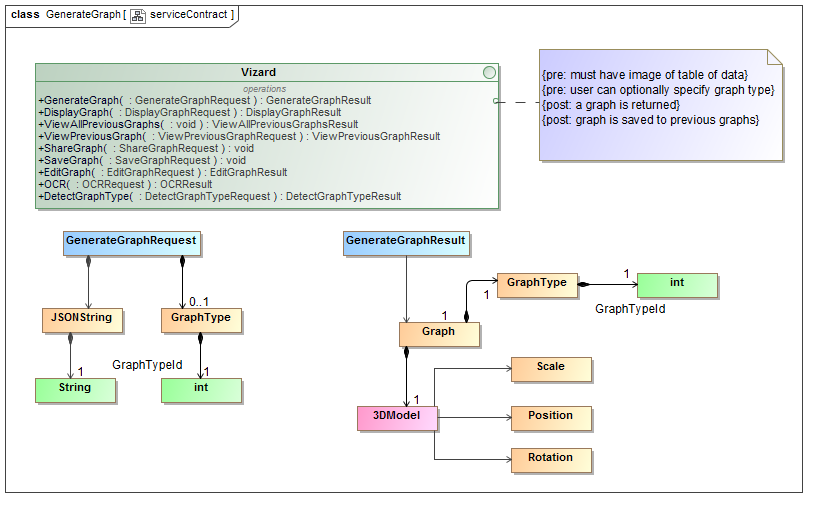
\includegraphics[width=\textwidth]{Images/class__GenerateGraph__serviceContract.png}  \\
		\caption{Services Contract : GenerateGraph}
	\end{figure}
	\begin{figure}[H]
		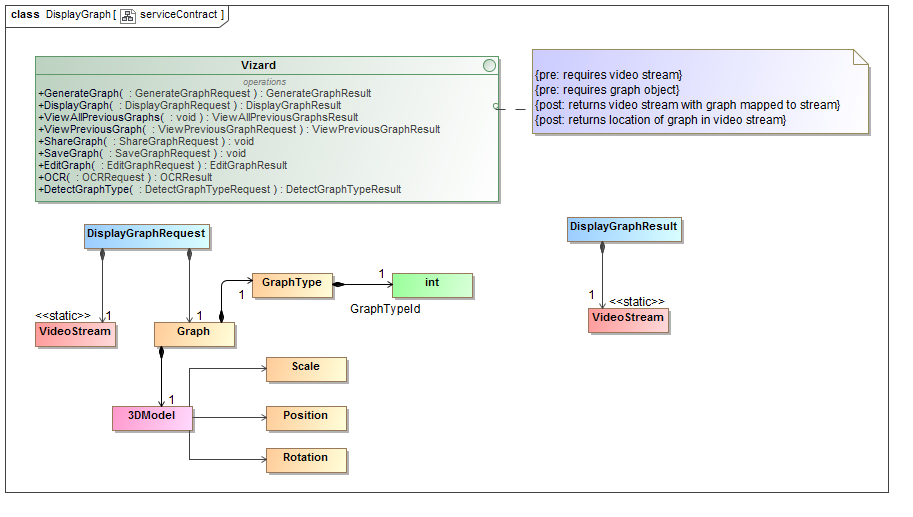
\includegraphics[width=\textwidth]{Images/class__DisplayGraph__serviceContract.png}  \\
		\caption{Services Contract : DisplayGraph}
	\end{figure}
	\begin{figure}[H]
		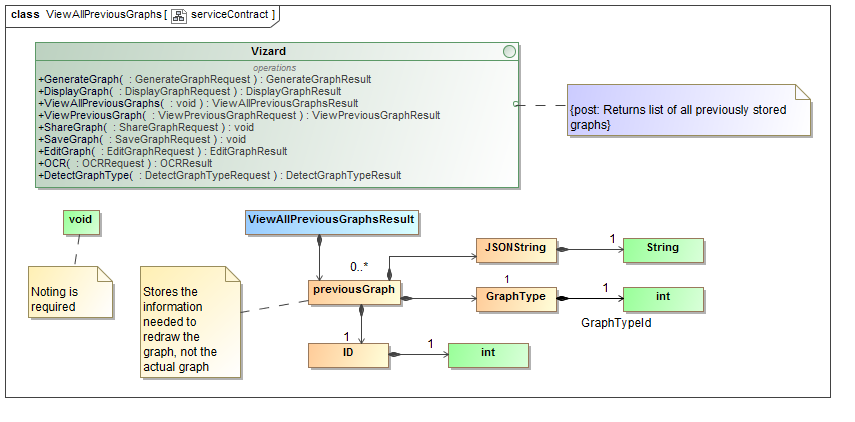
\includegraphics[width=\textwidth]{Images/class__ViewAllPreviousGraphs__serviceContract.png}  \\
		\caption{Services Contract : ViewAllPreviousGraphs}
	\end{figure}
	
	\begin{figure}[H]
		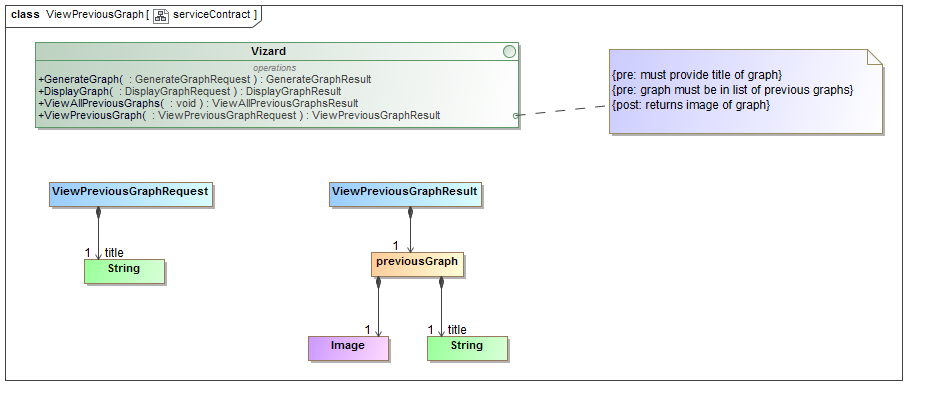
\includegraphics[width=\textwidth]{Images/class__ViewPreviousGraph__serviceContract.png}  \\
		\caption{Services Contract : ViewPreviousGraph}
	\end{figure}
	
	\begin{figure}[H]
		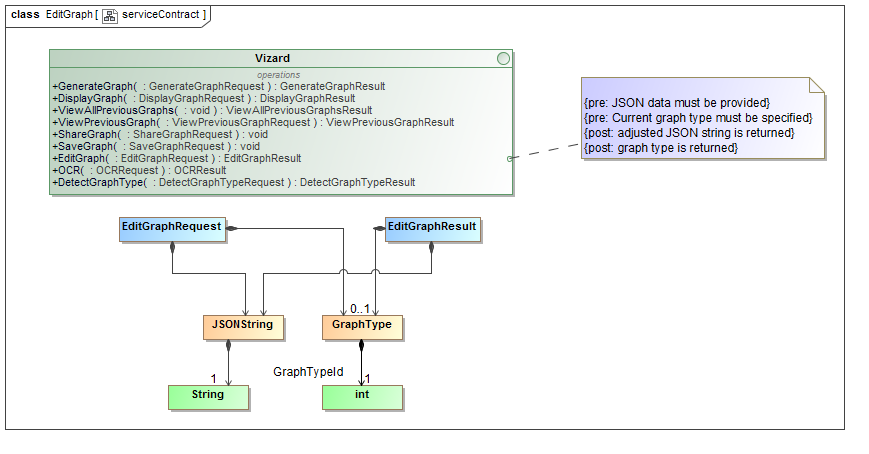
\includegraphics[width=\textwidth]{Images/class__EditGraph__serviceContract.png}  \\
		\caption{Services Contract : EditGraph}
	\end{figure}
	
	\begin{figure}[H]
		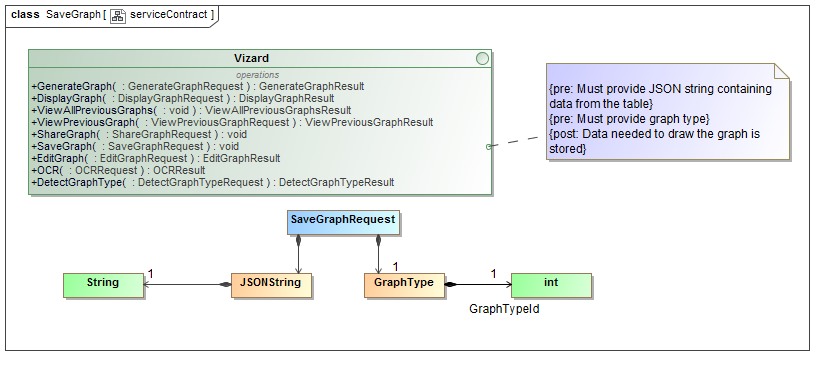
\includegraphics[width=\textwidth]{Images/class__SaveGraph__serviceContract.png}  \\
		\caption{Services Contract : SaveGraph}
	\end{figure}
	
	\begin{figure}[H]
		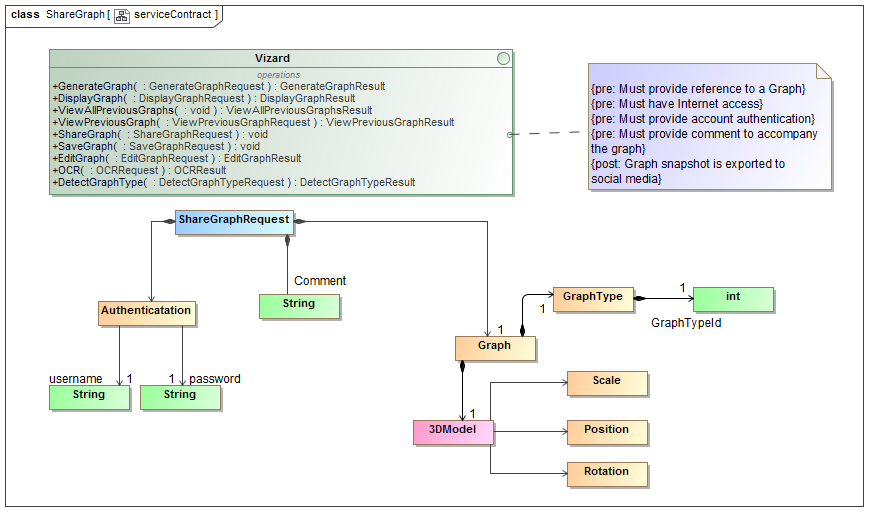
\includegraphics[width=\textwidth]{Images/class__ShareGraph__serviceContract.png}  \\
		\caption{Services Contract : ShareGraph}
	\end{figure}
	
	\begin{figure}[H]
		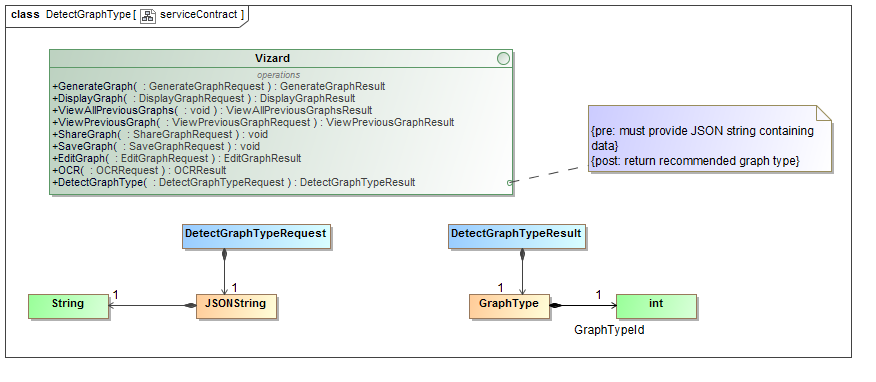
\includegraphics[width=\textwidth]{Images/class__DetectGraphType__serviceContract.png}  \\
		\caption{Services Contract : DetectGraphType}
	\end{figure}
	
	\begin{figure}[H]
		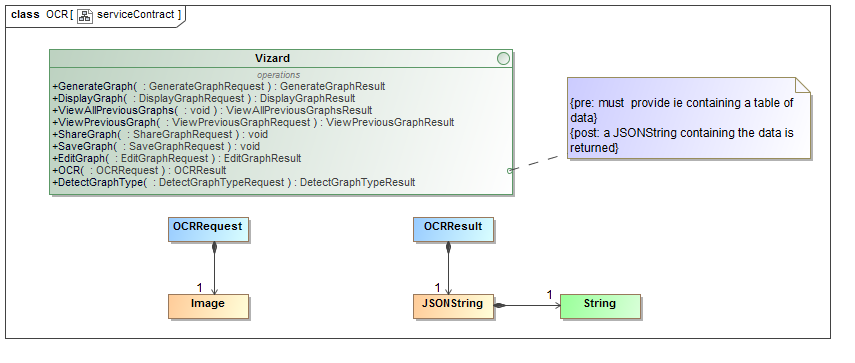
\includegraphics[width=\textwidth]{Images/class__OCR__serviceContract.png}  \\
		\caption{Services Contract : OCR}
	\end{figure}
\subsubsection{Global Scope}
\begin{figure}[H]
		\includegraphics[width=\textwidth]{Images/global_scope.png}  \\
		\caption{Use Case: Global Scope}
	\end{figure}
\subsection{Required functionality}
	\begin{figure}[H]
		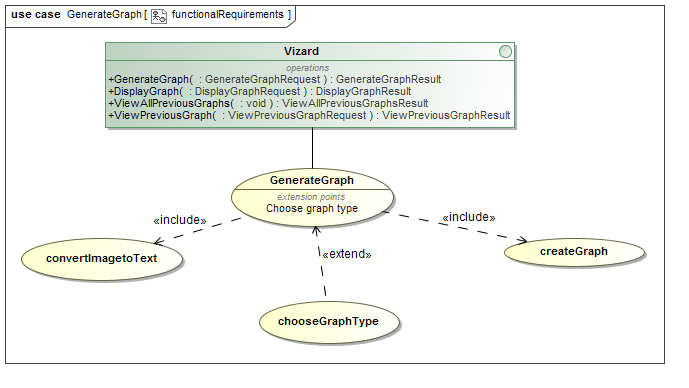
\includegraphics[width=\textwidth]{Images/uc__GenerateGraph__functionalRequirements.png}  \\
		\caption{Required functionality : GenerateGraph}
	\end{figure}
	\begin{figure}[H]
		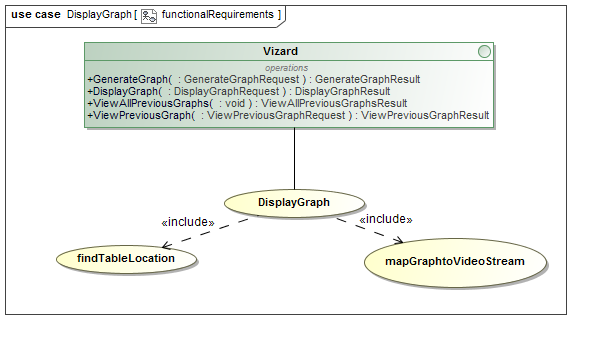
\includegraphics[width=\textwidth]{Images/uc__DisplayGraph__functionalRequirements.png}  \\
		\caption{Required functionality : DisplayGraph}
	\end{figure}
	\begin{figure}[H]
		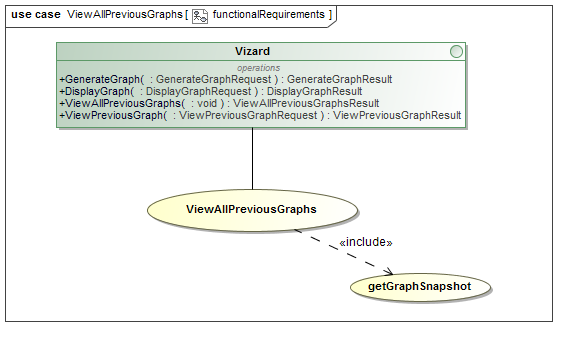
\includegraphics[width=\textwidth]{Images/uc__ViewAllPreviousGraphs__functionalRequirements.png}  \\
		\caption{Required functionality : ViewAllPreviousGraphs}
	\end{figure}
	\begin{figure}[H]
		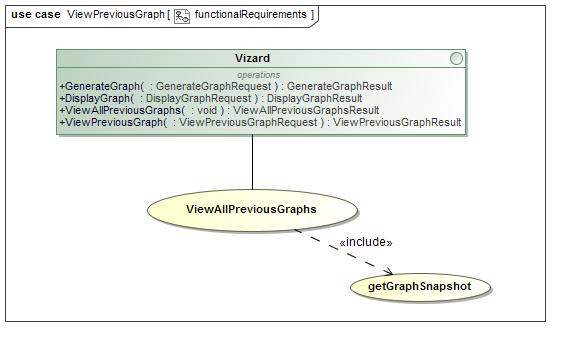
\includegraphics[width=\textwidth]{Images/uc__ViewPreviousGraph__functionalRequirements.png}  \\
		\caption{Required functionality : ViewPreviousGraph}
	\end{figure}	
	
	\begin{figure}[H]
		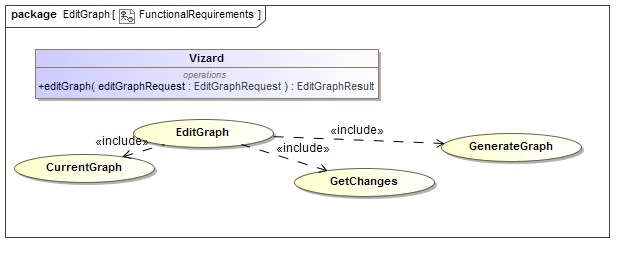
\includegraphics[width=\textwidth]{Images/uc__EditGraph}  \\
		\caption{Required functionality : EditGraph}
	\end{figure}
	
	\begin{figure}[H]
		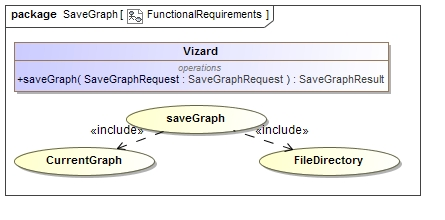
\includegraphics[width=\textwidth]{Images/uc__SaveGraph}  \\
		\caption{Required functionality : SaveGraph}
	\end{figure}
	
	\begin{figure}[H]
		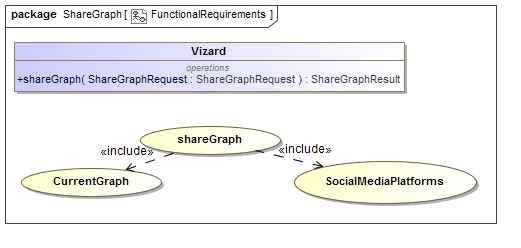
\includegraphics[width=\textwidth]{Images/uc__ShareGraph}  \\
		\caption{Required functionality : ShareGraph}
	\end{figure}


%\subsection{Domain Model}

%\subsection{Use of Reference Architectures and Frameworks}

%\subsubsection{Web 2.0 Reference Architecture}

%\subsection{Access and Integration Channels}

\newpage

\end{document}